%%%% Proceedings format for most of ACM conferences (with the exceptions listed below) and all ICPS volumes.
\documentclass[sigconf]{acmart}
%%%% As of March 2017, [siggraph] is no longer used. Please use sigconf (above) for SIGGRAPH conferences.

%%%% Proceedings format for SIGPLAN conferences 
% \documentclass[sigplan, anonymous, review]{acmart}

%%%% Proceedings format for SIGCHI conferences
% \documentclass[sigchi, review]{acmart}

%%%% To use the SIGCHI extended abstract template, please visit
% https://www.overleaf.com/read/zzzfqvkmrfzn


%%%%%%%%%%%%%%%%%%%%%%%%%%%%%%%%%%%%%%%%%%%%%%%%%%%%%%%%%%%%%%%%%%%%%%%%%%%%%%%%%%%%%%%%%%%%%%%%%%%%%%%%%%%%%%%%%%%%%%%%%%%%%%%%%%%%%%%%%%%%%%%%%%%%%%%%%
% PACKAGES
%%%%%%%%%%%%%%%%%%%%%%%%%%%%%%%%%%%%%%%%%%%%%%%%%%%%%%%%%%%%%%%%%%%%%%%%%%%%%%%%%%%%%%%%%%%%%%%%%%%%%%%%%%%%%%%%%%%%%%%%%%%%%%%%%%%%%%%%%%%%%%%%%%%%%%%%%
\usepackage{booktabs} % For formal tables
%% perso packages:
\usepackage{epstopdf}
\usepackage{microtype}
\usepackage{tabularx}
\usepackage{multirow}
%\usepackage{arydshln}
\usepackage{subfig}
\usepackage{balance}
\usepackage{caption}
\usepackage{graphicx}

%%%%%%%%%%%%%%%%%%%%%%%%%%%%%%%%%%%%%%%%%%%%%%%%%%%%%%%%%%%%%%%%%%%%%%%%%%%%%%%%%%%%%%%%%%%%%%%%%%%%%%%%%%%%%%%%%%%%%%%%%%%%%%%%%%%%%%%%%%%%%%%%%%%%%%%%%
% DOCUMENT's Identification
%%%%%%%%%%%%%%%%%%%%%%%%%%%%%%%%%%%%%%%%%%%%%%%%%%%%%%%%%%%%%%%%%%%%%%%%%%%%%%%%%%%%%%%%%%%%%%%%%%%%%%%%%%%%%%%%%%%%%%%%%%%%%%%%%%%%%%%%%%%%%%%%%%%%%%%%%
% Copyright
%\setcopyright{none}
%\setcopyright{acmcopyright}
%\setcopyright{acmlicensed}
\setcopyright{rightsretained}
%\setcopyright{usgov}
%\setcopyright{usgovmixed}
%\setcopyright{cagov}
%\setcopyright{cagovmixed}


% DOI
\acmDOI{10.475/123_4}

% ISBN
\acmISBN{123-4567-24-567/08/06}


%%%%%%%%%%%%%%%%%%%%%%%%%%%%%%%%%%%%%%%%%%%%%%%%%%%%%%%%%%%%%%%%%%%%%%%%%%%%%%%%%%%%%%%%%%%%%%%%%%%%%%%%%%%%%%%%%%%%%%%%%%%%%%%%%%%%%%%%%%%%%%%%%%%%%%%%%
% CONFERENCE
%%%%%%%%%%%%%%%%%%%%%%%%%%%%%%%%%%%%%%%%%%%%%%%%%%%%%%%%%%%%%%%%%%%%%%%%%%%%%%%%%%%%%%%%%%%%%%%%%%%%%%%%%%%%%%%%%%%%%%%%%%%%%%%%%%%%%%%%%%%%%%%%%%%%%%%%%
%Conference
\acmConference[ICMR 2018]{ACM Yokohama conference}{June 2018}{Yokohama, Japan} 
\acmYear{2018}
\copyrightyear{2018}

\acmArticle{4}%??
\acmPrice{15.00}%??

%%%%%%%%%%%%%%%%%%%%%%%%%%%%%%%%%%%%%%%%%%%%%%%%%%%%%%%%%%%%%%%%%%%%%%%%%%%%%%%%%%%%%%%%%%%%%%%%%%%%%%%%%%%%%%%%%%%%%%%%%%%%%%%%%%%%%%%%%%%%%%%%%%%%%%%%%
\begin{document}
%%%%%%%%%%%%%%%%%%%%%%%%%%%%%%%%%%%%%%%%%%%%%%%%%%%%%%%%%%%%%%%%%%%%%%%%%%%%%%%%%%%%%%%%%%%%%%%%%%%%%%%%%%%%%%%%%%%%%%%%%%%%%%%%%%%%%%%%%%%%%%%%%%%%%%%%%

%%%%%%%%%%%%%%%%%%%%%%%%%%%%%%%%%%%%%%%%%%%%%%%%%%%%%%%%%%%%%%%%%%%%%%%%%%%%%%%%%%%%%%%%%%%%%%%%%%%%%%%%%%%%%%%%%%%%%%%%%%%%%%%%%%%%%%%%%%%%%%%%%%%%%%%%%
% TITLE
%%%%%%%%%%%%%%%%%%%%%%%%%%%%%%%%%%%%%%%%%%%%%%%%%%%%%%%%%%%%%%%%%%%%%%%%%%%%%%%%%%%%%%%%%%%%%%%%%%%%%%%%%%%%%%%%%%%%%%%%%%%%%%%%%%%%%%%%%%%%%%%%%%%%%%%%%
\title{Annotating, understanding, and predicting long-term video memorability}
%\titlenote{}
%\subtitle{}
%\subtitlenote{}

%%%%%%%%%%%%%%%%%%%%%%%%%%%%%%%%%%%%%%%%%%%%%%%%%%%%%%%%%%%%%%%%%%%%%%%%%%%%%%%%%%%%%%%%%%%%%%%%%%%%%%%%%%%%%%%%%%%%%%%%%%%%%%%%%%%%%%%%%%%%%%%%%%%%%%%%%
% AUTHORS
%%%%%%%%%%%%%%%%%%%%%%%%%%%%%%%%%%%%%%%%%%%%%%%%%%%%%%%%%%%%%%%%%%%%%%%%%%%%%%%%%%%%%%%%%%%%%%%%%%%%%%%%%%%%%%%%%%%%%%%%%%%%%%%%%%%%%%%%%%%%%%%%%%%%%%%%%
%author 1
%\author{Romain Cohendet}
%\authornote{}
%\orcid{1234-5678-9012}
%\affiliation{%
%	\institution{Technicolor}
%	\streetaddress{Technicolor Research \& Licensing, 975 Avenue des Champs Blancs, 35576 Cesson-Sevigne, France}
%	\city{Rennes} 
%	\state{France} 
%	\postcode{}
%}
%\email{romain.cohendet@technicolor.com}

%author 2
%\author{Karthik Yadati}
%\affiliation{%
%	\institution{University of Delft}
%	\streetaddress{}
%	\city{Delft} 
%	\state{} 
%	\postcode{}
%}
%\email{N.K.Yadati@tudelft.nl}

%author 3
%\author{Ngoc Khanh Duong}
%\affiliation{%
%	\institution{Technicolor}
%	\city{Rennes} 
%	\country{France}}
%\email{Quang-Khanh-Ngoc.Duong@technicolor.com}

%author 4
%\author{Claire-Helene Demarty}
%\affiliation{%
%	\institution{Technicolor}
%	\city{Rennes}
%	\country{France}
%}
%\email{Claire-Helene.Demarty@technicolor.com}

%%%%%%%%%%%%
%%% for blind review %%%
%author 1
\author{Removed for review}
%author 2
\author{Removed for review}
%author 3
\author{Removed for review}
%author 4
\author{Removed for review}


% The default list of authors is too long for headers.
\renewcommand{\shortauthors}{R. Cohendet et al.}

%%%%%%%%%%%%%%%%%%%%%%%%%%%%%%%%%%%%%%%%%%%%%%%%%%%%%%%%%%%%%%%%%%%%%%%%%%%%%%%%%%%%%%%%%%%%%%%%%%%%%%%%%%%%%%%%%%%%%%%%%%%%%%%%%%%%%%%%%%%%%%%%%%%%%%%%%
% ABSTRACT
%%%%%%%%%%%%%%%%%%%%%%%%%%%%%%%%%%%%%%%%%%%%%%%%%%%%%%%%%%%%%%%%%%%%%%%%%%%%%%%%%%%%%%%%%%%%%%%%%%%%%%%%%%%%%%%%%%%%%%%%%%%%%%%%%%%%%%%%%%%%%%%%%%%%%%%%%
\begin{abstract}
The growing number of video contents on the Internet encourages us to find new ways to make more relevant their occurrences in our everyday life.
In this context, memorability can be regarded as a useful metric of video importance to help us make a choice between competing videos.
However, the research on computational understanding of video memorability is in its early stages.
There is no available dataset for modelling purposes, and the few previous attempts provided protocols not generalizable to collect data at a large scale.
Furthermore, the video computational features valuable to build a robust memorability predictor remain largely undiscovered.
In this article, we propose a new protocol to collect long-term memorability annotations, that we use to measure memory performances of 104 participants from weeks to years after memorization.
We then analyze the data collected for 660 videos by focusing on its quality, and test it against different characteristics such as response time, duration of memory retention and repetition of visualization.
We finally conduct an extensive feature analysis, comparing several methods and classes of features, to propose a computational model for the prediction of video memorability.
\end{abstract}

%%%%%%%%%%%%%%%%%%%%%%%%%%%%%%%%%%%%%%%%%%%%%%%%%%%%%%%%%%%%%%%%%%%%%%%%%%%%%%%%%%%%%%%%%%%%%%%%%%%%%%%%%%%%%%%%%%%%%%%%%%%%%%%%%%%%%%%%%%%%%%%%%%%%%%%%%
%% NEW ACM TAXONOMY to categorise ACM article
%%%%%%%%%%%%%%%%%%%%%%%%%%%%%%%%%%%%%%%%%%%%%%%%%%%%%%%%%%%%%%%%%%%%%%%%%%%%%%%%%%%%%%%%%%%%%%%%%%%%%%%%%%%%%%%%%%%%%%%%%%%%%%%%%%%%%%%%%%%%%%%%%%%%%%%%%
\begin{CCSXML}
	<ccs2012>
	<concept>
	<concept_id>10010520.10010553.10010562</concept_id>
	<concept_desc>Computer systems organization~Embedded systems</concept_desc>
	<concept_significance>500</concept_significance>
	</concept>
	<concept>
	<concept_id>10010520.10010575.10010755</concept_id>
	<concept_desc>Computer systems organization~Redundancy</concept_desc>
	<concept_significance>300</concept_significance>
	</concept>
	<concept>
	<concept_id>10010520.10010553.10010554</concept_id>
	<concept_desc>Computer systems organization~Robotics</concept_desc>
	<concept_significance>100</concept_significance>
	</concept>
	<concept>
	<concept_id>10003033.10003083.10003095</concept_id>
	<concept_desc>Networks~Network reliability</concept_desc>
	<concept_significance>100</concept_significance>
	</concept>
	</ccs2012>  
\end{CCSXML}

%\ccsdesc[500]{Computer systems organization~Embedded systems}
%\ccsdesc[300]{Computer systems organization~Redundancy}
%\ccsdesc{Computer systems organization~Robotics}
%\ccsdesc[100]{Networks~Network reliability}

%%%%%%%%%%%%%%%%%%%%%%%%%%%%%%%%%%%%%%%%%%%%%%%%%%%%%%%%%%%%%%%%%%%%%%%%%%%%%%%%%%%%%%%%%%%%%%%%%%%%%%%%%%%%%%%%%%%%%%%%%%%%%%%%%%%%%%%%%%%%%%%%%%%%%%%%%
% KEYWORDS
%%%%%%%%%%%%%%%%%%%%%%%%%%%%%%%%%%%%%%%%%%%%%%%%%%%%%%%%%%%%%%%%%%%%%%%%%%%%%%%%%%%%%%%%%%%%%%%%%%%%%%%%%%%%%%%%%%%%%%%%%%%%%%%%%%%%%%%%%%%%%%%%%%%%%%%%%
\keywords{Video memorability, Long-term memory, Measurement protocol, Memorability scores, Deep learning, Multimedia information retrieval}

%%%%%%%%%%%%%%%%%%%%%%%%%%%%%%%%%%%%%%%%%%%%%%%%%%%%%%%%%%%%%%%%%%%%%%%%%%%%%%%%%%%%%%%%%%%%%%%%%%%%%%%%%%%%%%%%%%%%%%%%%%%%%%%%%%%%%%%%%%%%%%%%%%%%%%%%%
%% ABOUT ICMR'2018 article...
%%%%%%%%%%%%%%%%%%%%%%%%%%%%%%%%%%%%%%%%%%%%%%%%%%%%%%%%%%%%%%%%%%%%%%%%%%%%%%%%%%%%%%%%%%%%%%%%%%%%%%%%%%%%%%%%%%%%%%%%%%%%%%%%%%%%%%%%%%%%%%%%%%%%%%%%%
\maketitle
%if we want the text be called from there
 %\input{samplebody-conf}

%% About the ICMR article on Media retrieval with VM
	% focus on "Multimedia content-based retrieval"
	% Length: from 6 to 8 pages + 1 additional page for references (no longer distinction between long and short papers)
	% Submission deadline: 2018/01/20
	% Contributions addressing the challenges of large-scale search and user behavior analysis are especially welcome

%%%%%%%%%%%%%%%%%%%%%%%%%%%%%%%%%%%%%%%%%%%%%%%%%%%%%%%%%%%%%%%%%%%%%%%%%%%%%%%%%%%%%%%%%%%%%%%%%%%%%%%%%%%%%%%%%%%%%%%%%%%%%%%%%%%%%%%%%%%%%%%%%%%%%%%%%
\section{Introduction}%nb of sections %2 PAGES
%%%%%%%%%%%%%%%%%%%%%%%%%%%%%%%%%%%%%%%%%%%%%%%%%%%%%%%%%%%%%%%%%%%%%%%%%%%%%%%%%%%%%%%%%%%%%%%%%%%%%%%%%%%%%%%%%%%%%%%%%%%%%%%%%%%%%%%%%%%%%%%%%%%%%%%%%
%opening
Enhancing the relevance of multimedia occurrences in our everyday life requires to imagine new ways to organize -- in particular, to retrieve -- digital contents.
Like other metrics of video "importance", such as aesthetics or interestingness, memorability can be regarded as useful to help us make a choice between competing videos.
In addition, memorability has the advantage of being clearly definable and objectively measurable (i.e., using a measure that is not influenced by the observer's personal judgment).
Thus, memorability has initially be defined as the probability for an image to be recognized \textbf{a few minutes} after a single view, when presented amidst a stream
of images \cite{isola_2011_makes}.
This definition has been widely accepted within subsequent work (e.g., \cite{mancas_2013_memorability,kim_2013_relative,celikkale_2013_visual,khosla_2015_understanding,lahrache_2016_bag}).

%from images to VM
The computational understanding of video memorability (VM) follows on from the study of image memorability prediction which has attracted increasing attention from the 2001 seminal work of Isola \textit{et al.} \cite{isola_2011_makes}.
With the recent introduction of deep learning to address the challenge of image memorability prediction, models also achieved very good results \cite{khosla_2015_understanding,baveye_2016_deep,squalli_2017_deep}.
As a result of this success, researchers have recently extended this challenge to the videos.
However, to the best of our knowledge, only two available studies focused on VM prediction \cite{han_2015_learning,shekhar_2017_show}.

%explain the scarcity of studies on VM
Several problems could explained this scarcity of studies.
Firstly, there is no publicly available dataset to train and test models.
This is probably the most serious obstacle to the rapid expansion of the VM prediction's search field.
Accordingly, to provide researchers with ground truth data should be our very first objective, similarly with the work of \cite{isola_2011_makes} and \cite{khosla_2015_understanding} which have enabled research on image memorability to flourish.
The second point is closely related to the first one: there is no widely accepted definition of VM.
The previous attempts to predict VM \cite{han_2015_learning,shekhar_2017_show} were based on different measures of memorability.
Furthermore, contrary to images, videos do not constitute clearly defined units.
They have supplementary dimensions -- sound and movement -- that critically contribute to the semantic and emotional information conveyed.
If harmonized, the videos used and the way memorability is measured will have a critical impact on what we will understand by VM.
The definition of image memorability by \cite{isola_2011_makes} had a great impact on subsequent work as aforementioned.
But it also inevitably limited researchers.
In particular, in previous research image memorability corresponds to memory performances measured only a few minutes after memorization.
But these might be poor predictors of longer term memory performances (at least in some instances; e.g., for emotional images \cite{cohendet_2016_prediction}).
Thus, VM data would benefit from a protocol that would measure lasting long-term memory performance.

%modelling
Regarding modelling, our capacity to propose efficient computational models is also important to meet the challenge of VM prediction. 
The previous attempts at predicting VM \cite{han_2015_learning,shekhar_2017_show} shed light on several features which have a predictive power of VM.
However, videos contain a great volume of data which can be used for feature extraction purposes, and the work is far for complete.

%objectives of the present study
The aim of this article is to participate in the expansion of the VM prediction emerging search field.
In particular, we:
\begin{itemize}
	\item propose a new protocol that measures very long-term memory performances (from weeks to years after memorization) to collect quality ground truth data (section 2);
	\item assess and analyze the collected data to better understand VM (section 3);
	\item model VM in an attempt to understand which computation features are better for this task (section 4).
\end{itemize}
In the next subsection, we review previous work on image and video memorability prediction, focusing on protocol and modelling questions.

%%%%%%%%%%%%%%%%%%%%%%%%%%%%%%%%%%%%%%%%%%%%%%%%%%%%%%%%%%%%%%%%%%%%%%%%%%%%%%%%%%%%%%%%%%%%%%%%%%%%%%%%%%%%%%%%%%%%%%%%%%%%%%%%%%%%%%%%%%%%%%%%%%%%%%%%%
\subsection*{Previous work}
%%%%%%%%%%%%%%%%%%%%%%%%%%%%%%%%%%%%%%%%%%%%%%%%%%%%%%%%%%%%%%%%%%%%%%%%%%%%%%%%%%%%%%%%%%%%%%%%%%%%%%%%%%%%%%%%%%%%%%%%%%%%%%%%%%%%%%%%%%%%%%%%%%%%%%%%%
\subsection{Measurement of memorability}
%Images work -- towards a long-term memorability
Almost all studies on image memorability prediction made use of one or the other of the two available large datasets designed specifically to meet this challenge \cite{isola_2011_makes,khosla_2015_understanding}.
To build these datasets, the authors, possibly constrained by the difficulty in conducting long crowdsourcing studies, measured memory performance a few minutes after memorization to obtain their memorability annotations.
As proposed in \cite{cohendet_2016_prediction}, this could be a problem if we conceive that memorability reflects a lasting memory performance.
Indeed, it has long been shown that long-term memories continue to change long after their memorization through an ongoing process called consolidation, which lasts weeks to years \cite{mcgaugh_2000_memory}.
%In particular, the early work of the psychologist Ebbinghaus showed that the drop in long-term memory performance in recall follow an exponential decay, and is particularly strong in the few days immediately following the memorization \cite{ebbinghaus_1913_memory}.
Because several factors influence the consolidation process (e.g., emotions, sleep, re-evocation), which does not equally affect all memories, the order of memorability ratings measured for videos is susceptible to change over time \cite{cohendet_2016_prediction}.
A protocol to collect memorability annotations would benefit from the capacity to capture long-lasting memory performances, averaged to obtain what we will later refer to as "long-term memorability".

%Han et al.
To our knowledge, the first attempt at predicting VM had been proposed by \cite{han_2015_learning}. 
The authors partially adapted the protocol proposed by \cite{isola_2011_makes} to measure image memorability for videos.
In contrast to the "memory game" proposed by Isola \textit{et al.} to collect memorability data, their protocol is however much heavier.
They used a classical recognition task to measure memory for videos, which consists in two steps: a free viewing task, followed two days later by a recall task.
The task duration, for each of the 20 participants, was about 24 hours, spread over 10 sessions (five free viewing tasks and five recall tasks) of about two hours each.
The authors used the same proportion of fillers (i.e., non repeated videos) in the free viewing and recall tasks (i.e., 4/5 of fillers and 1/5 of repeated videos named targets) to, according to them, guarantee that viewers were unaware of targets.
If it was mandatory in \cite{isola_2011_makes} for which encoding and recall tasks were interlaced, there is here a way to alleviate the task without impacting its quality; indeed, reducing the number of fillers in the free viewing task would have very little impact on the memorability scores (often authors even use only material interrogated later in the learning/free viewing task).
Furthermore, as pointed by \cite{shekhar_2017_show}, the long time span of the experiment makes difficult the generalization of this protocol, in particular to build an extensive dataset.
Furthermore, authors measure memory after two days, but the consolidation process lasts weeks to years: it would be interesting to collect even longer term memory performance measures.

%Shekhar et al.
Another earlier approach was the one of \cite{shekhar_2017_show}.
The participants performed a crowdsourcing experiment consisted of a free viewing task where they saw a sequence a videos, followed by a recall task for which they had to answer textual question (such as: "Did you see a man juggling?", "Did you see a car on a road?").
The major drawback of the study comes from the use of questions instead of a classic visual recognition task.
Indeed, the memorability scores computed for the videos may reflect not only the differences in memory performances but also the differences between the questions in terms of difficulty
The authors have tested complexity of textual questions, but their measure is not sufficient to represent the real difficulty of the question in its complexity (ease of understanding, in particular for the non-anglophone people that works with Amazon Mechanical Turk, ease of imaging, ease to retrieve a scene by some words more the by others...).
Especially since the authors took into account the response time of the participants to calculate the memorability scores of the videos.
One will note that this potential bias could have also affected the measure of inter-human consistency.
Furthermore, the questions are handcrafted, and the choices for types of questions and videos are very limited (e.g., the question "Did you see a car on a road?" implies that in a whole experimental session one can have just one car on a road).
The authors also manually ensured that no textual questions nor videos in a session were similar in content.
This makes it difficult to generalize this protocol to the construction of an extensive dataset.

\subsection{Memorability modelling}
%intro on focus on features to discover
Previous attempts at predicting image and video memorability highlighted quite a few features that correlates with memorability.

%image memorability prediction
The pioneering work of Isola \textit{et al.} focused primarily on building computational models to predict image memorability from low-level visual features \cite{isola_2011_makes}.
It appeared from this first attempt that it is possible to predict to some extent the degree of picture's memorability.
Several characteristics have been found to be relevant for predicting memorability in subsequent work, for example saliency features \cite{mancas_2013_memorability}, interestingness and aesthetic \cite{isola_2014_makes}, or emotions \cite{khosla_2015_understanding}.
The best results was finally obtained by using fine-tuned deep features, which outperformed all other features in \cite{khosla_2015_understanding}, reaching a rank correlation of $.64$ which is near human consistency ($.68$) measured for ground truth collected in the study.
This result was confirmed in \cite{baveye_2016_deep,squalli_2017_deep}.

%VM prediction
Regarding the VM prediction, Han \textit{et al.} propose a method which combines the power of audiovisual and fMRI-derived features \cite{shekhar_2017_show}.
They preliminary built a computational model learned with fMRI features, which supposedly convey the brain activity of memorizing videos, which enable them to finally predict VM without fMRI scans.
However, the method would be difficult to generalize 

Shekhar \textit{et al.} conducted a performance analysis of several computationally extracted features before building their memorability predictor \cite{shekhar_2017_show}.
The analysis encompassed C3D deep learning feature for video classification, video semantics obtained thanks to video captioning method, saliency features, dense trajectories, and color features.
They found that the most predictive feature combination used video semantics, spatio-temporal, saliency and color features.
The feature that performed the best when tested alone was video semantics.
The authors used a captioning method to generate a semantic description of the videos.
The text generated by this method was then processed by a recursive auto-encoder network that outputted a 100-dimensional representation of the videos.
Due to the particularity of the dataset of Shekhar \textit{et al.} -- that is, their aforementioned use of questions to measure memorability --, it would be interesting to confirm if this combination works equally well on another dataset, and in particular if images captioning features also perform the best.

%%%%%%%%%%%%%%%%%%%%%%%%%%%%%%%%%%%%%%%%%%%%%%%%%%%%%%%%%%%%%%%%%%%%%%%%%%%%%%%%%%%%%%%%%%%%%%%%%%%%%%%%%%%%%%%%%%%%%%%%%%%%%%%%%%%%%%%%%%%%%%%%%%%%%%%%%
\section{Memorability dataset construction}
%%%%%%%%%%%%%%%%%%%%%%%%%%%%%%%%%%%%%%%%%%%%%%%%%%%%%%%%%%%%%%%%%%%%%%%%%%%%%%%%%%%%%%%%%%%%%%%%%%%%%%%%%%%%%%%%%%%%%%%%%%%%%%%%%%%%%%%%%%%%%%%%%%%%%%%%%
\subsection{Video collection}
%why did we choose movie
We wanted our protocol to measure memory performance after a significant retention period.
This can be achieved either with a longitudinal study, or by measuring a memory created prior to the experiment.
We chose the latter because it enabled us to immediately measure very long-term memory.
Thus, the main characteristic of the proposed protocol, in contrast with previous work, is the absence of learning (often, free viewing) task, replaced by a questionnaire designed to collect information about the participants' prior memory.

%movies and videos selections
 %with HD or dvdrip quality, in orginal (i.e.,english) version, without without subtitles [add if results HD vs. DVDrip]
We first established a list of 100 movies, taking care to mix popularity and genres.
We then manually selected seven videos of 10 seconds from each movie.
To maintain a high intra-video semantic cohesion, we did not make cuts that would impair the understanding of the scene, nor did we aggregate shots that belong to different scenes.
Indeed, since the semantics is linked to the memorability of images \cite{isola_2014_makes}, we can expect it is linked to the memorability of videos too.

%neutral vs. typical
We also gave preference to the videos we called "neutral", by contrast to the "typical" ones.
According to our definition, a neutral video is a part of a movie which contains no element that would enable someone to easily guess it belongs to a particular movie.
The list of undesirable elements includes but is not limited to: recognizable famous actors, typical music, style, etc.
Typical videos are simply defined as non-neutral videos.
In most movies, just a few or no 10-sec neutral videos exist.
That explains why we obtained only 127 neutral videos for 573 typical ones (while we expected two neutral and five typical videos per movie).
 
%%%%%%%%%%%%%%%%%%%%%%%%
\subsection{Annotation protocol}
%presentation protocol
The protocol is composed of two tasks.
Firstly, participants had to fill a questionnaire intended to collect data about whether they know the 100 selected movies.
Secondly, participants performed a recognition task on videos selected from their responses to the questionnaire.

%participants, facilities and apparatus
104 participants ($22-58$ years of age; $\mu_{age}=37.1 $; $\sigma_{age}=10.4$; $26\%$ of them female), mostly educated persons (engineers or researchers mainly), participated in the experiment on a volunteer basis.
The experiment was taking place in a room insulated from noise and equipped with subdued lights.
The videos, of HD or DVD quality, were displayed on a 60 inch monitor (Sony Bravia).
The participants were seated at a distance of about 220 centimeters from the screen (that is three times the screen height).

%questionnaire
Having provided basic demographics, participants filled out a questionnaire on the selected movies.
For each of them, they were asked whether they remembered watching fully the movie.%Each item included a movie poster with its name below, followed by the question.
In case of a positive answer, three additional questions followed on: 1/ their confidence of watching the movie (Not confident / slightly confident / 50\% confident / considerably confident / 100\% confident), 2/ the duration since they saw the movie (less than month / 1 year / 5 years / 10 years / more than 10 years), and 3/ the number of times they saw the movie (once / 2-4 times / 5-9 times / 10-19 times / more than 20 times).
In case of a negative answer, only one question followed on, relating to their confidence of not having seen the movie.
The questionnaire required about 20 minutes to complete.

%Algorithm selection
Based on the answers to the questionnaire, an algorithm selected 80 targets and 40 fillers (i.e. videos from never seen movies) among the movies associated with the highest degree of certitude, with a maximum of two videos from the same movie.
Another selection criterion was the videos' number of annotations, so that it was balanced.

%Recognition task
The questionnaire was followed by the recognition task itself, in which participants saw the 120 randomly chosen 10-seconds videos, separated by an inter-stimuli interval of 2 seconds.
They had to press the space bar when they recognized a video in particular, and not when they guessed that the particular video came from a movie they had seen (which was possible only for the typical videos).
In case a participant pressed the space bar, the video continued until its end.

%%%%%%%%%%%%%%%%%%%%%%%%
\subsection{Memorability scores calculation}
%first discuss why we filtered the data from 700 to 660 and give other statistics.
After collecting the data, we kept only the 660 videos that had been seen at least 4 times as targets (from the initial set of 700 videos).
On average, each video of our dataset has been viewed as a target by $10.7$ participants; which corresponds to the mean number of observations that enter in the calculation of a memorability score.
Each video has also been viewed as a filler by $10.5$ participants.

%Then explain how the scores are computed
We then assigned a memorability score to each video, defined as the correct recognition rate of the video.
The average percentage of correct detections for all participants was $46.71\%$ ($\sigma=14.65\%$), and the average false alarm (i.e., answer on a filler) rate was $4.16\%$ ($\sigma=5.27\%$).
Figure \ref{fig:response_time_vs_memorability}(a) provides a distribution of the videos according to their degree of memorability.

%%%%%%%%%%%%%%%%%%%%%%%%%%%%%%%%%%%%%%%%%%%%%%%%%%%%%%%%%%%%%%%%%%%%%%%%%%%%%%%%%%%%%%%%%%%%%%%%%%%%%%%%%%%%%%%%%%%%%%%%%%%%%%%%%%%%%%%%%%%%%%%%%%%%%%%%%
\section{Study of the memorability annotations}
%%%%%%%%%%%%%%%%%%%%%%%%%%%%%%%%%%%%%%%%%%%%%%%%%%%%%%%%%%%%%%%%%%%%%%%%%%%%%%%%%%%%%%%%%%%%%%%%%%%%%%%%%%%%%%%%%%%%%%%%%%%%%%%%%%%%%%%%%%%%%%%%%%%%%%%%%
In this section, we conduct an analysis of the ground truth data collected thanks to the protocol described in the previous section.
We firstly focus on quality of data through a human consistency on memorability analysis, and by comparing neutral videos with typical videos.
We then test the data against different characteristics such as response time, duration of memory retention and repetition of visualization.
In what follows, error bars in the graphs correspond to standard error of the mean, $\mu$ to the mean, $\sigma$ to the standard deviation ans $N$ to the number of observations in the statistics.

%%%%%%%%%%%%%%%%%%%%%%%%
\subsection{Consistency analysis}
%global consistency calculation
We implemented the method proposed in \cite{isola_2014_makes} to measure the human consistency.
We randomly split our 104 participants into two independent halves, and calculate how well video memorability scores from the first half of the participants match with video memorability scores from the second half of the participants.
Averaging over 25 random half-split trials, we calculated a Spearman's rank correlation $\rho$ of $0.57$ between these two sets of scores.

%Fig Consistency
 %Histogram of number of nb of videos per possibble nb of annotations
 %Curve of human consistency
\begin{figure}[!htbp]
	\centering
	\subfloat[]{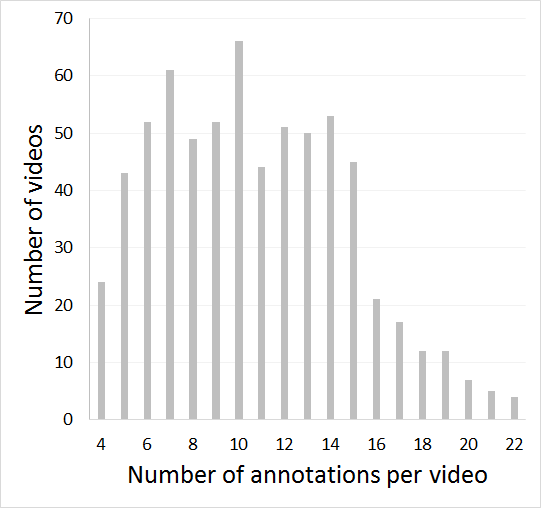
\includegraphics[width=0.45\columnwidth]{figures/histogram_nb_sequences_for_nb_of_annotations.png}}
	\quad
	\subfloat[]{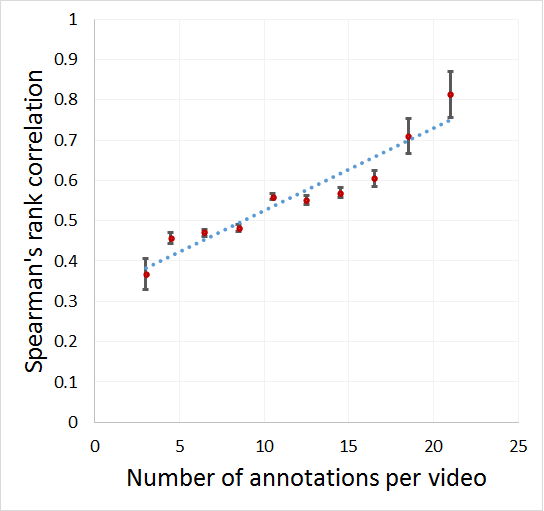
\includegraphics[width=0.45\columnwidth]{figures/Measure_of_human_consistency.png}}
	\quad
	\caption{\label{fig:human_consistency}(a) Number of videos for each possible number of annotations per video. (b) Human consistency averaged over 25 random splits obtained using the method proposed by \cite{isola_2014_makes} (with linear trendline).}
\end{figure}

%per nb of annotations consistency %comparison with image memorability
We reproduced this calculation to obtain 25 Spearman's correlation coefficients as a function of the mean number of annotations per video, presented in figure \ref{fig:human_consistency}(b).
This curve is to be compared with the histogram presented in figure \ref{fig:human_consistency}(a), which shows that the number of videos for each number of annotations was unequal.
According to the curve, we achieved a mean consistency of $.70$ from about 18 annotations, which is consistent with the previous attempt of \cite{han_2015_learning}.
$.70$ corresponds also to the maximum consistency obtained when collecting image memorability scores \cite{isola_2011_makes,khosla_2015_understanding}, but for a much bigger number of annotations (80) per image.
It must be noted that the protocols are different between the image memorability experiments conducted in \cite{isola_2011_makes,khosla_2015_understanding} and ours or the work in \cite{han_2015_learning}.
We conducted a measure of long-term memory performance after at least two days of memorization, whereas in \cite{isola_2011_makes,khosla_2015_understanding} it is measured after a dozen of seconds to a few minutes. 
In addition, VM annotations were collected through in-lab experiments, and images annotations through crowdsourcing experiments.
These factors might have contributed to the shortest number of annotations necessary to reach a high human consistency for videos.
However, it would be interesting in the future to confirm if an important difference exists between images and videos regarding the number of annotations necessary to achieve a high human response consistency.
Apart from the conclusions we could draw about the universality of the intrinsic memorability of videos compared to images, this would mean that the magnitude of the work to carry out to build an extensive database for VM prediction is substantially smaller than one could expect from work on image memorability prediction.

%%%%%%%%%%%%%%%%%%%%%%%%%%%%%%%%%%%%%
\subsection{Neutral and typical videos}
In our experiment, participants were given clear instructions that they had to really recognize any video they were presented as already seen, and not only guess that a video was coming from a movie which title was proposed in the questionnaire.
We perform an analysis to compare neutral videos, which contain no element that would enable participants to guess that a video belongs to a particular movie, and typical videos.
Indeed, if neutral videos received objective answers from participants, it might be more subjective for typical videos, that could be more or less easily related to the movie they belong to.

A Wilcoxon rank-sum test indicated that the memorability was greater for neutral ($Mdn=.2, \mu=.24$) than for typical ($Mdn=.53, \mu=.53$) videos, $Z=10.22, p<.00001$.
Apart from the subjectivity aspect, we expected such a result because neutral videos contain less contextual elements, useful for recognition.
Thus, this result does not necessarily mean that participants tended to guess -- rather to purely recognize -- videos drawn from movies they have seen.

A Wilcoxon rank-sum test indicated that the human consistency on memorability was slightly greater for neutral ($Mdn=.44, \mu=.45$) than for typical ($Mdn=.40, \mu=.41$) videos, $Z=2.75, p<.01$.
Along with the comments collected from the participants, who have as a majority reported difficulty to know if they were guessing or really recognizing the videos, this result suggests that human congruency is higher for more 'objectively' recognized segments than for ones with subjectivity as part of the equation. 
One could note there is probably not just pure subjectivity here, but also a bias: some participants could have helped themselves with the context.
If confirmed, this would constitute a weakness of our protocol to collect extensive data, that one should in that case counteract by adapted measures of control.

We can also note that the false alarm rate was low for neutral videos ($\mu=.05$) as well as for typical videos ($\mu=.03$).
Specifically, we expect lucky confusions to account for little of correct detections on average for the two sorts of videos.

%%%%%%%%%%%%%%%%%%%%%%%%%%%%%%%%%%%%%
\subsection{Response time}
%figure Distribution of memorability scores + Mean response time vs. degrees of memorability
\begin{figure}[!htbp]
	\centering
	\subfloat[]{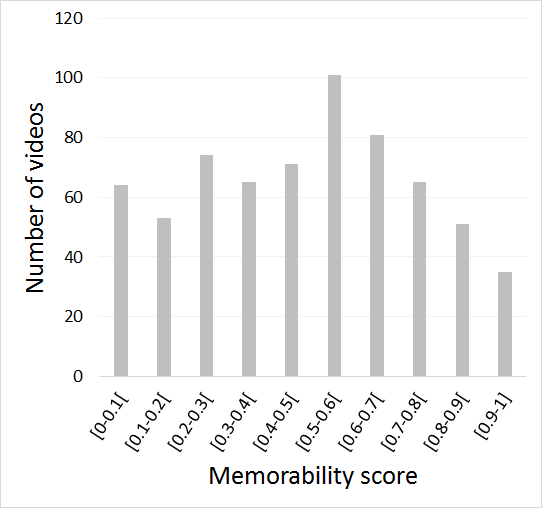
\includegraphics[width=0.45\columnwidth]{figures/memorability_scores_distribution.png}}
	\quad
	\subfloat[]{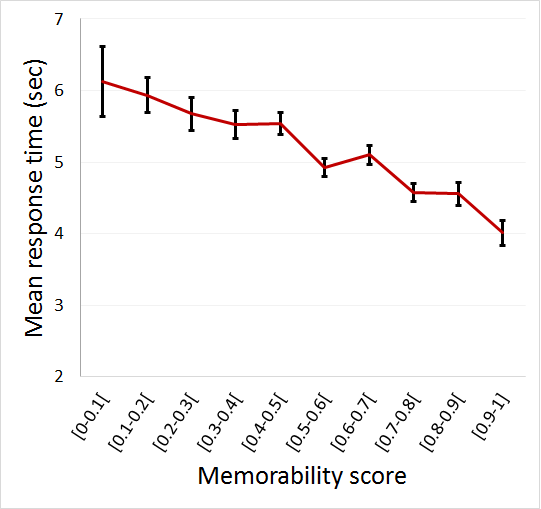
\includegraphics[width=0.45\columnwidth]{figures/Response_time_vs_Memorability.png}}
	\quad
	\caption{\label{fig:response_time_vs_memorability}(a) Distribution of the memorability scores. (b) Mean response time for correct recognitions against videos' memorability scores.}
\end{figure}
%(a) Sample of the dataset with key frames of videos sorted from most memorable (left) to less memorable (right).

Figure \ref{fig:response_time_vs_memorability} (b) shows that the response time to do a correct detection decreases when the memorability of the video increases.
We also observed a Pearson's correlation of $-0.36$ ($p<.0001$) between the response time on the targets and their memorability scores.
These two results indicate that participants tended to answer quicker when the videos were more memorable, even though the participants did not receive any instruction to answer quickly.
This suggests that people tend to naturally answer rapidly after having recognized the video.
This also suggests either that the most memorable videos are also the most accessible in memory, and/or that the most memorable videos contain more early recognizable elements than the less memorable ones.
In \cite{shekhar_2017_show}, the response time of the participants was taken to be the measure of video memorability.
The authors chose this measure to avoid a long gap between viewing and recall stage.
Our results validate -- to some extent -- their modus operandi: the fact that response time decreases linearly when the memorability increases suggest that the response time is a good indicator of the memorability of the videos (at least, in a recognition task). 
 %However, the linear continuous decrease in response time when memorability score values increase supports the first hypothesis: one can hardly imagine that the early recognizable elements (e.g., the face of a person, a particular place...) decreases linearly with the memorability of our 10-sec semantically consistent videos.
 %The hypothesis of a linear relation between the accessibility of the videos in memory and their memorability is consistent with the associative functioning of long-term memory \cite{tulving_1974_cue}.
 %Information stored in long-term memory is retrieved by way of association with other memories.
 %One can hypothesize that the memorability of a video depends on how interconnected with peoples' prior memory the memories of this video is: in our experiment, the most memorable videos would have been the most easily accessible in memory, thus the most rapidly retrieved.
%target vs. fillers
 %We observed no significant correlation ($r=-0.09, p=.276$) between the mean response time to do a false alarm and the memorability score of the sequence.
 %In conjunction with our previous hypothesis, only early recognizable elements could have played a role if we had observed such a correlation, not the accessibility in memory (because fillers are, by definition, videos that are not in memory).
 %Let us imagine that the videos' early recognizable elements explain alone that the most memorable videos are recognized quickly than the less memorable ones.
 %If we assume that recognizable elements are responsible of the false alarms by misleading the participants, we could have expected that early recognizable elements would have encouraged the participants to wrongly recognized fillers quickly when they were most memorable, since, as was suggested, people tend to naturally answer rapidly after having recognized the video.
 %But we observed no effect of early recognizable elements on response time for fillers, while we observed an effect of either this factor of accessibility in memory for targets, in the same conditions (outside of this factor).
 %This suggests that the presence of early recognizable elements does not explain the relation we observed between the response time and the memorability of the target videos, and thus that the hypothesis of the accessibility in memory is better.
%response time for correct recognitions vs. false alarms 
 %A Wilcoxon rank-sum test indicated that the response time was greater to do a correct recognition ($Mdn=4.5, \mu=4.88 sec$) than to do a false alarm ($Mdn=5.8, \mu=5.90 sec$), $Z=-5.10, p<.00001$.
 %One explanation is that participants tended to hesitate more before generating a false alarm than when correctly recognizing a target.
 %It points out the fact that memories of videos are generally not obvious but more blurred.
 %This is an interesting point to connect with the fact that human consistency is lower for typical than for neutral videos: because of the non obviousness of if they had memories or not, the part of subjectivity for typical videos could have fostered participants to answer when they hesitated if they were guessing that a video came from a movie they had seen or remembering it.
 %The higher degree of memorability of typical videos compare to the one for neutral videos could be partly due to this factor too.
 %Among other, this is also an argument in favour of the most "objective" possible measure to choose to constitute an extensive dataset for VM prediction.

%%%%%%%%%%%%%%%%%%%%%%%%%%%%%%%%%%%%%
\subsection{User context and memorability}
To provide us with an estimation context-related factors collected through our questionnaire, we processed to a logistic regression, using demographics and answers to the questionnaire as regressors, and the detection of a target video (with two possible discrete outcomes, detected or not) as observations to fit.
Regarding the participants' nationality, we grouped them into occidental (69 pers) and non-occidental (35 pers) categories, motivated by our use of occidental movies, which could have more meaning for occidental than for non-occidental people.
We also tested age and gender to reveal a potential bias in our movies' choice, maybe more interesting for people of a certain age and gender.
The results of the logistic regression are shown in Figure \ref{fig:logistic_regression} (a).
The method also provides a measure of the statistical significance of each feature in the model through their \textit{p}-value.

The model, in case of a single observation, can be written as:
\begin{equation}
	y_n=\beta_0 + \sum\limits_{k=1}^K x_{nk} \beta_k+\epsilon_n
\end{equation}
where $y$ is the dependent variable -- the probability to correctly recognize a video --, $x$ are our predictor values, $\beta$ are the coefficients to be estimated, and $\epsilon$ indicates the error term.

%figure logistic regression (a), and movie last viewing and nb of viewing (b)
\begin{figure}[!htbp]
	\centering
	\subfloat[]{\includegraphics[width=0.75\columnwidth]{figures/logistic_regression.png}}
	\\
	%\subfloat[]{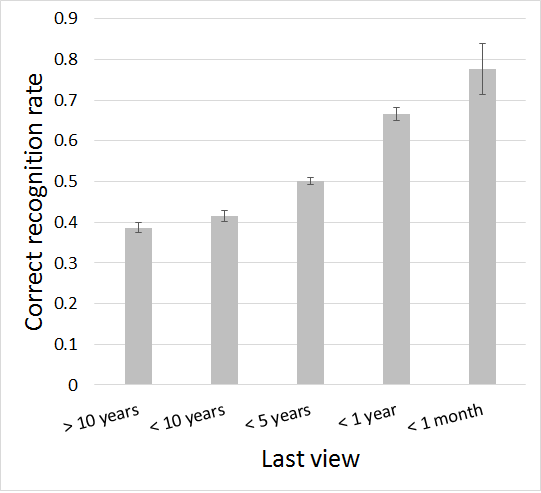
\includegraphics[width=0.45\columnwidth]{figures/film_last_viewing.png}}
	\quad
	\subfloat[]{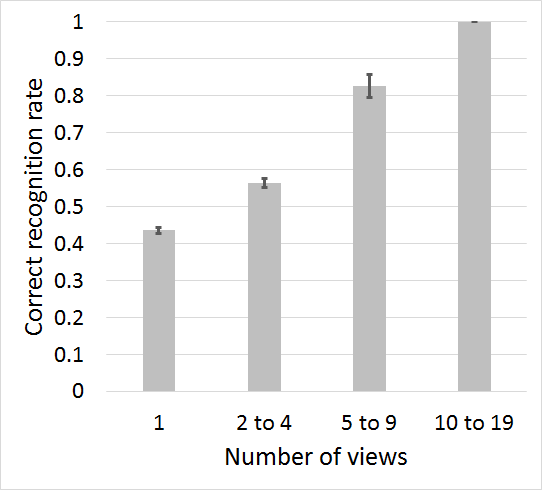
\includegraphics[width=0.45\columnwidth]{figures/nb_of_viewing.png}}
	\quad
	\caption{\label{fig:logistic_regression}(a) Features regression coefficients for the probability of detecting the repetition of a video (Features significance: *$p<.0001$). (b) Mean memorability depending on when occurred the last viewing, and (c) how many times the movie had been seen.}
\end{figure}

%memorability change over time
Firstly, the retention duration is highly negatively correlated with the probability to recognize a video.
Figure \ref{fig:logistic_regression} (b) shows that this decrease in memory for videos over time is continuous.
This result indicates that long-term memory of videos continue to be altered over times for years.
It implies that a memorability score, to provide an accurate representation of an average long-term memory performance, should correspond to a memory measure carried out as late as possible after the memorization.

%memorability and viewving repetition
Secondly, the number of views is highly correlated with the probability to recognize a video.
As expected, the more a movie was seen, the better the videos were memorized.
Figure \ref{fig:logistic_regression} (c) shows that this continues to be true even with more than 9 viewings.
(However, the number of observations was very low (12) for videos which belongs to movies with 10 or more views.)
One should note that the repetition of a viewing could not be the (only) factor involved in the above phenomenon; in particular, viewing again a movie may be the sign of a special interest which would explained a better memorization (e.g., via a greater attentional and emotional investment).
The fact remains that repetition is an important factor to ask people when measuring their prior memory.
Furthermore, a protocol used to build an extensive database for VM prediction should, in case of multiple measures of memory (e.g., after the memorization and then after a longer delay), avoid measuring twice the same items, because this repetition could artificially increase the performance measured for the last items.

%Ajouter Age et expliquer que les movies sont plutôt jeune génération -- donner corrélation Age*Memorability => pas possible
According to Figure \ref{fig:logistic_regression} (a), we observed no significant effects of the demographic factors (nationality, age and gender).
This suggests that the videos were about equally susceptible to be recognized by the different participants (or, that the relations between these factors and the observations are too complex to have been captured by the model).

%%%%%%%%%%%%%%%%%%%%%%%%%%%%%%%%%%%%%
% Other results possible
%%%%%%%%%%%%%%%%%%%%%%%%%%%%%%%%%%%%%
%\subsection{Mean memorability of the videos compare to the movie they come from}
	%Corriger score par moyenne de mem du movie -- est-ce que ça a un sens ? Par le nombre de vue du movie ? par le moment où il a été vu?

%\subsection{Quality of the movies}
	%dvdrip vs. HD 720-1080 => Difference of memorability? => Interesting

%\subsection{movie genre and IMDB ratings}
	%test the momorability od the videos compare to the mean one of the movie.
	%Correct bu the mean participant's performance
	%And maybe other IMDB annotations/labels

%\subsection{Context}
	%Analyse the context (order of video presentation) influent the memo: to be check if we have enough information?
	%Une vidéo par rapport à toutes les autres différentes à un impact sur sa mem ?
	%S'inspirer de la technique de Bylinskii
	%tester la mémorability de séquences très proches (prise à intervalles très proche + vérif = même scène)

%\subsection{Features linked to memorability}
	%tester ces features comme dans 'What makes a photograph...'
	% Indoor/Outdoor, low-level visal feautures (color... -- i.e., as in isola et al.), salinecy maps

%\subsection{Indoor \textit{.vs} outdoor scenes}
	%indoor/outdoor comme isola et al. mais en contrecarrant l'effet de la couleur -- car ils expliquent que c'est par la corrrélation entre couleur et mémorabilité est expliqué par le fait que les couleurs plus froides sont d'exté.

%\subsection{Other points}
	%add other relevant points found in MIT papers e.g.,

%Corr Evolution of the memorability along time for videos scores
%Use order positions for that (e.g., mean memorability for position 1, 2... 120)


%%%%%%%%%%%%%%%%%%%%%%%%%%%%%%%%%%%%%
%\subsection{New manner to compute memorability scores: take into account time and FA}
%Une nouvelle manière pour prendre en compte les FA dans les scores de mémorabilité applicable à l'étude de la mémorabilité sur les images
%Ce qui à la fin de cette section vient avant permet de conclure cette partie en disant : la meilleure façon de calculer les scores de mémorabilité, c'est comme ça.
% The question here is: "Must we correct our memorabiliy scores by taking into account the mean memorability of the participants --> No, of the movie --> No' --> So the point here is just to provide an overview.

%%%%%%%%%%%%%%%%%%%%%%%%%%%%%%%%%%%%%%%%%%%%%%%%%%%%%%%%%%%%%%%%%%%%%%%%%%%%%%%%%%%%%%%%%%%%%%%%%%%%%%%%%%%%%%%%%%%%%%%%%%%%%%%%%%%%%%%%%%%%%%%%%%%%%%%%%
\section{Memorability prediction} %for Khartik
\label{mem-pred}
%%%%%%%%%%%%%%%%%%%%%%%%%%%%%%%%%%%%%%%%%%%%%%%%%%%%%%%%%%%%%%%%%%%%%%%%%%%%%%%%%%%%%%%%%%%%%%%%%%%%%%%%%%%%%%%%%%%%%%%%%%%%%%%%%%%%%%%%%%%%%%%%%%%%%%%%%
Until now, we have presented the video collection and the annotation protocol. 
%We then computed memorability scores and analyzed how different users fared in remembering the video sequences from the movies they have already watched.
In this section, we move towards building a machine learning model that can learn and then predict the VM score of a video from its audio-visual features.
The main goal of modelling is to understand if VM is predictable, and if yes identify which features: generic, perceptual, or semantic, are suitable for such prediction.
We pose the problem as a standard regression problem and Figure \ref{prop-apprch} illustrates different steps in our method.
%First, we see that the videos are converted into feature vectors and then a regression model is trained that can in-turn predict the memorability scores for new videos.
In the following sub-sections, we explain our choice of features and models to address the problem in hand.

\begin{figure}[h]	  
  \centering
    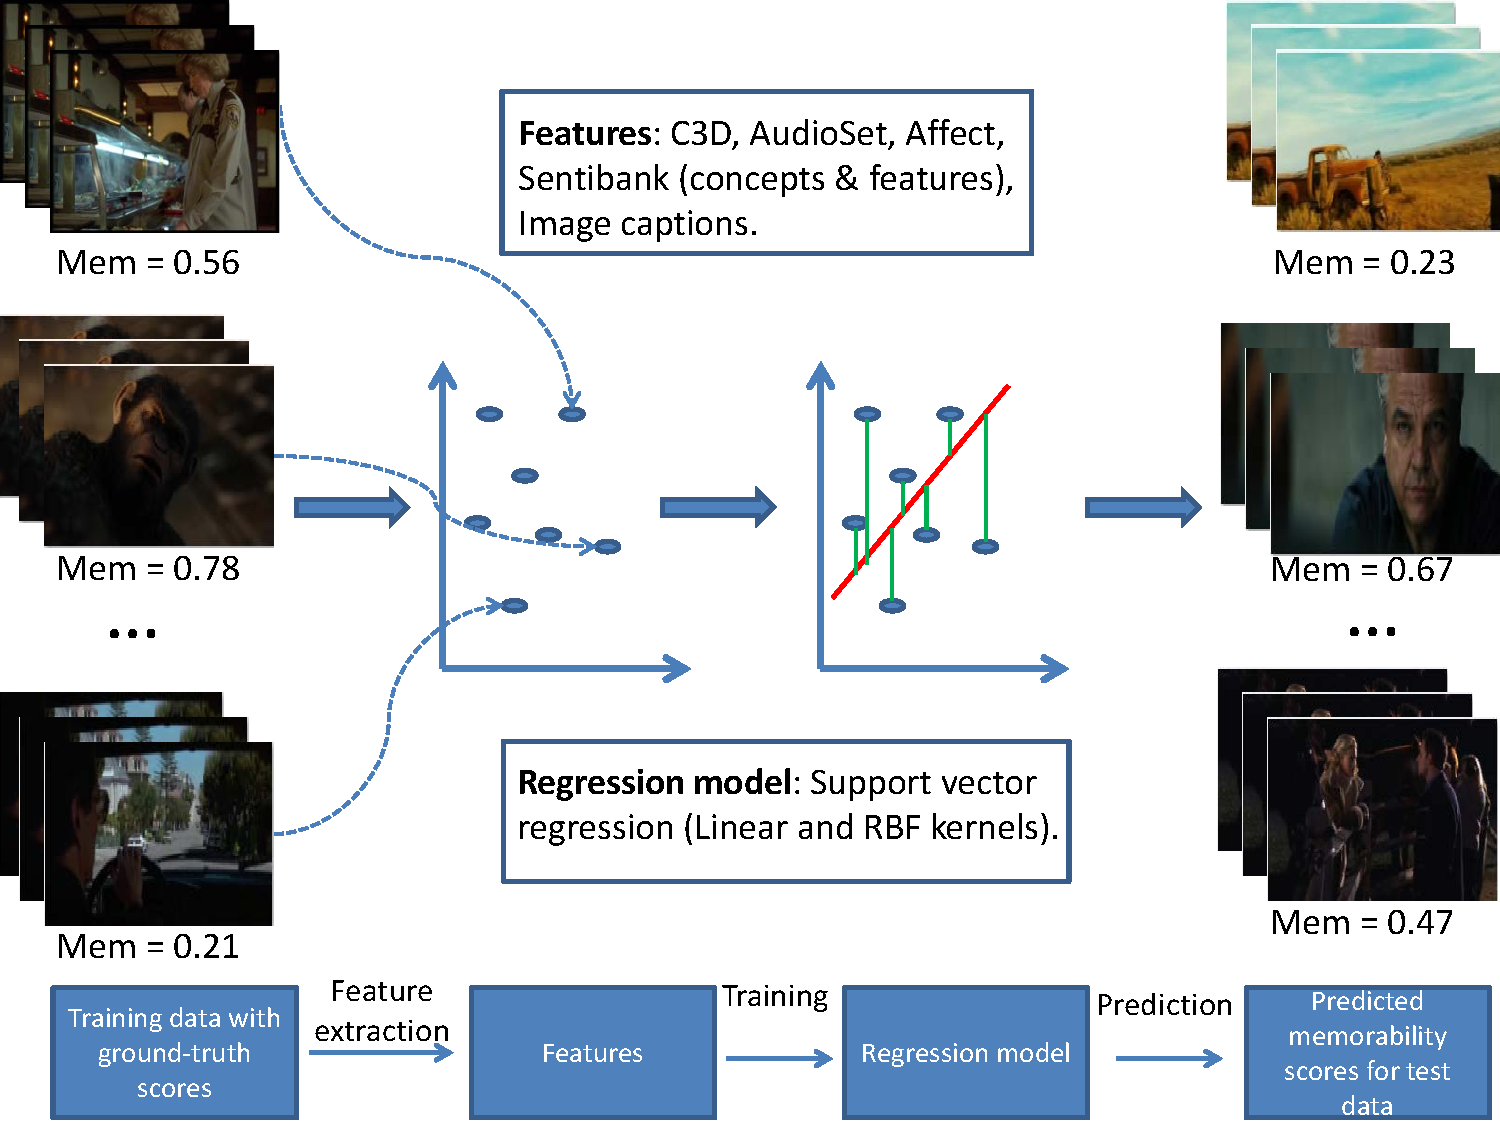
\includegraphics[width=0.9\columnwidth]{figures/approach.pdf}
		\caption{Proposed approach for memorability score prediction.}
    \label{prop-apprch}
\end{figure}

%Before we go into the technical details about the different audio-visual features and regression models we explored, we will talk about how we split our dataset.
To build our predictive model, we split the dataset, at the level of movies, into training (70\%), validation (15\%) and test (15\%) data, which translates into 70 movies in the training set and 15 movies each in the validation and test sets.
We chose to split our dataset at the level of movies, instead of the videos, in order to avoid videos from the same movie being present in the training as well as the evaluation (validation+test) set.

\subsection{Feature extraction}
\label{feat-extr}
%We explore a variety of audio-visual features in building a model that can predict memorability scores for new videos.
The task of remembering a specific video has a high cognitive complexity in general, suggesting that it requires a semantic understanding of the content and/or some other perceptual factors such as the emotion conveyed by the video. 
Many users who participated in our experiments indicated that it is a difficult task.
While trying to build a machine learning model for such a task, we explore different kinds of features that can be extracted from the audio-visual signal.
We investigate a variety of generic state-of-the-art features (\cite{c3d-feat}, \cite{audioset-feat}) and compare them with other semantic (\cite{caption-feat}) and perceptual (emotion) features (\cite{sb-feat}).

%We mostly stick to state-of-the-art deep learning features that have been proposed in vision and audio research communities for tasks like video classification \cite{c3d-feat}, event detection \cite{audioset-feat}, image captioning \cite{caption-feat}, and concept detection \cite{sb-feat}. 

\subsubsection{Spatio-temporal visual features (C3D)}
\label{c3d-feat}
These features are extracted from the C3D model, a 3-dimensional convolutional network proposed for generic video analysis \cite{c3d-feat}. 
The main motivation to use C3D is that it encodes both the spatial and temporal information in the video.
The model has been proposed for video analysis and is not an extension of a model for image analysis, unlike other state-of-the-art models like VGG16 \cite{vgg16}.
We use the publicly available model trained on the Sports-1M dataset \cite{c3d-feat} and extract the output of the fully connected layer -- fc6 of the network with a dimensionality of 4096.
We additionally explore the use of principal component analysis (PCA) (named C3D (PCA) in Table \ref{res-4-10-ann}) for the dimension reduction, as the original dimensionality is very high when compared to other features.

\subsubsection{Audio features (AudioSet)}
\label{as-feat}
Using a recently released AudioSet \cite{audioset-feat} model, which was trained on a large dataset for event detection, we extract 128-dimensional embeddings for each audio track associated with a video in our dataset.
We use these embeddings for training the regression models.
The motivation to use these features is that they are state-of-the-art in the audio event detection research and events could play a major role in how people remember sequences in movies.
Additionally, we wanted to investigate how the audio channel contributes to building a model for VM prediction.

\subsubsection{Emotion related features (SentiBank and Affect)}
\label{emo-feat}
As research in psychology showed that emotion and memory are correlated \cite{emo-mem}, we investigate the use of emotion-related feature in our prediction system.
For modelling emotion from the visual content, we resort to a visual sentiment concept detector: SentiBank \cite{sb-feat}.
SentiBank is a set of 1200 trained visual concept detectors providing a mid-level representation of sentiment from visual content.
We use the binary code for concept detection, from images, provided by the authors.
The SentiBank concept detector provides two pieces of information: concepts with probabilities and features.
Concepts are adjective--noun pairs and the probability represents how likely each concept is depicted visually in an image.
Examples of some concepts in the SentiBank ontology are: \emph{young driver}, \emph{scary face}, \emph{terrible pain}, etc.

We sample one frame for every second of the video in our dataset, resulting in 10 frames per video.
We run the SentiBank concept detector on each of these 10 frames and rank the concepts based on the probability of their occurrence in the frame and take the top-50 concepts.
We extract a 300-dimensional word2vec \cite{word2vec} embeddings, for each of the 50 concepts and take an average to obtain a single vector per frame.
We repeat this process for all the 10 frames and take the average of all the vectors to obtain a single feature vector for each video.
Sentibank detectors also provide a 4096-dimensional features for each frame and we take the average across all the frames to obtain one 4096-dimensional feature vector for each video.
In the end, we use a 300-dimensional concept vector and a 4096-dimensional feature vector.

In addition to SentiBank concepts, we investigate other ways to capture emotional content in a video. 
Following a circumplex model of affect (the experience of emotion) \cite{affect-model}, we define arousal as the dimension of affect that measures the excitement in the video, while valence measures whether the video invokes positive or negative emotion.
We resort to an audio-visual analysis of the video to obtain its arousal and valence scores using the method described in \cite{affect}.
For each frame in the video, we compute the arousal and valence scores using the method proposed in \cite{affect}.
In order to keep a fixed dimensionality of the feature vector, we take the first 200 frames in the video because of the varying frame rates across the videos.
We concatenate the arousal and valence scores for the first 200 frames in each video resulting in a 400-dimensional feature vector (200 for arousal and 200 for valence) for a video.

\subsubsection{Visual semantic features (Image captions)}
\label{sem-feat}
Visual semantics are known to play an important role in image memorability (\cite{sem-mem}, \cite{squalli_2017_deep}).
We utilize the state-of-the-art research in image captioning to capture such high-level semantics of the video \cite{caption-feat}.
We sample one frame for every second of the video in our dataset, resulting in 10 frames per video.
For each of these 10 frames, we run the caption detector (code provided by the authors) and obtain a caption for the frame.
For each non-functional word in the caption, we extract a 300-dimensional word2vec \cite{word2vec} embeddings and take an average of all the words to obtain a single vector per frame.
We repeat this process for all the 10 frames and take the average of all the vectors to obtain a single 300-dimensional feature vector for each video.

\subsection{Modelling and evaluation}
\label{model-eval}
We use the features discussed in Section \ref{feat-extr} to train a Support Vector Regression (SVR) model with two different kernels (linear and RBF) for the VM score prediction. 
We use the grid search strategy to obtain the best hyper-parameters for SVR: $C$ = $\{0.1, 1, 10, 100, 1000\}$ and $\gamma$ = $\{0.01, 0.1, 1, 10, 100\}$.
We use the standard regression metric: Mean Squared Error ($MSE$) for the optimization process.
The choice of SVR is guided by the small size of the dataset. 
We have chosen to go with the same regressor for all the features because our focus was mainly on identifying which features are more important for VM prediction. 
This way we ensure that the difference in performances is because of the features themselves.

%Since we are posing the memorability prediction problem as a regression problem, we use the standard regression metric: Mean squared error ($MSE$) for evaluation.
We use the spearmann correlation ($SpCorr$) to measure the rank correlation between the predicted memorability scores and the ground-truth.
We chose this particular metric as it gives us an indication of how close the predicted memorability scores are to human labelled ground-truth memorability scores.

In addition to the variety of features explained in Section \ref{feat-extr}, we also explore a combination of all the features by concatenating them into a single feature vector.
While performing such a concatenation, we use the lower dimensional features for C3D and SentiBank features, obtained after applying PCA to the original set.
%Each of the videos in our dataset has multiple annotations and we pick sequences with at least 4 annotations for training the models.
%In this way, we eliminate movies that were not seen by a majority of the users who participated in our experiment.
%Since we are using an SVR with linear and rbf kernels, we train the models on the training set (70 movies) and validate the model on the validation set (15 movies), before reporting the final scores on the test set (15 movies).
We pick the SVR model parameters: kernel (linear or RBF), $C$ and $\gamma$ that give the best performance on the validation set.
We retrain the model with these parameters using the training set and evaluate on the final test set.
In the experiments where we use a dimension reduction method (PCA) for C3D and SentiBank features, we retain 95\% of variance in the data while reducing the feature dimensions. 

\subsection{Memorability prediction results}
\label{pred-res}
In this section, we will discuss how the models trained on different features perform in predicting memorability scores of new videos.
We report the results of the prediction on both the validation and test sets.
We also report only correlation scores: $SpCorr$ and not $MSE$ keeping in mind the space constraints.
Additionally, $SpCorr$, which provides a rank correlation between the predicted and the ground-truth memorability scores, is more informative.
We compute the average number of annotations per video in the train and test set for both the cases ($geq$ 4 and $geq$ 8 annotations).
We observe that the number of annotations in the train and test sets are balanced and there is no mismatch.
For example, each sequence in the test set has around 10 annotations while there are 9 annotations for each sequence in the training on an average.

Table \ref{res-4-10-ann} reports the the results of prediction capability of the model trained on different features.
There are two sets of results reported in the table: $SpCorr$ ($\geq$ 4 annotations) and $SpCorr$ ($\geq$ 8 annotations).
The first set of results correspond to the prediction capability of the model when trained on videos with at least 4 annotations and the second set corresponds to the results when trained on videos with at least 8 annotations.
We will further discuss why we report the results with the model trained on videos with at least 8 annotations.

Observing the first set of results in Table \ref{res-4-10-ann}, we can clearly see that the image captions and C3D occupy the top-2 places in terms of performance on the test set. 
Image captions capture the visual semantics in the video, while C3D features encode the visual spatio-temporal information.
These results are consistent with previous results on predicting image memorability \cite{squalli_2017_deep}.
Our dataset consists of videos taken from movies that have a specific story-line; semantics and spatio-temporal information seem to be playing an important role in people remembering specific scenes from movies.

Other features like AudioSet come close to the performance of the above features (third best feature), but only audio signal does not seem to be enough for predicting video memorability.
Another observation from Table \ref{res-4-10-ann} is that the combination of all the features (last row in the table) does not appear in the top-3 best performing features.
One of the reasons for this could be that there is a lot of redundance when combining all the features into a single feature vector.
In future, we could look at selectively combining the features to investigate if that improves the performance. 

One of our initial hypotheses was that emotion would play an important role in VM, supported by literature from psychology \cite{emo-mem}.
Please recall that we used different set of features to encode the emotion in a video: Affect \cite{affect} and SentiBank \cite{sb-feat}.
Observing the scores in Table \ref{res-4-10-ann}, we can say that the SentiBank features (fourth row from bottom) perform slightly better than the affect features (sixth row from bottom).
But the models trained on image captioning features clearly out-perform those trained on emotion features.
This could be because of the following reasons: our choice of features to capture emotion related information is not suitable for our task, or the performance of the emotion prediction models is not good enough for memorability prediction, or we are not able able to establish the correlation between emotion and memorability because of the limited size of our dataset.
%From the analysis on this dataset and the features we used for capturing emotion related information, we \emph{cannot} conclude that emotion plays an important role in memorability.
%In the future, we could investigate more robust emotion/affect prediction models to confirm that both emotion and memorability are correlated as suggested in the literature \cite{emo-mem}.

We further investigate the effect of the number of annotations, for videos in the training set, on the performance of the model.
%Based on our experimental results, we observe that the image captioning feature performs the best while using training videos that have at least 4 annotations.
%For this purpose, we train different SVR models with varying number of annotations on the training set using image captioning features only.
We train a model, using image captioning features, on training sequences with at least 4 annotations and use this model to predict the memorability score for videos in the validation set.
We repeat this process for different number of annotations per video in the training set: from 4 to 15 annotations.
Please note that the validation set in each of the repetitions is fixed and only the training set changes.
We provide a demonstration of how $SpCorr$ varies with an increasing number of annotations in the training set in Figure \ref{num-ann}.
We observe that $SpCorr$ first increases up to 5 annotations and then remains constant before decreasing (beyond 8 annotations).
In the wake of this observation, we investigate the performance of all the features when we train the regression model with videos that have at least 8 annotations.

\begin{figure}[h]	  
  \centering
    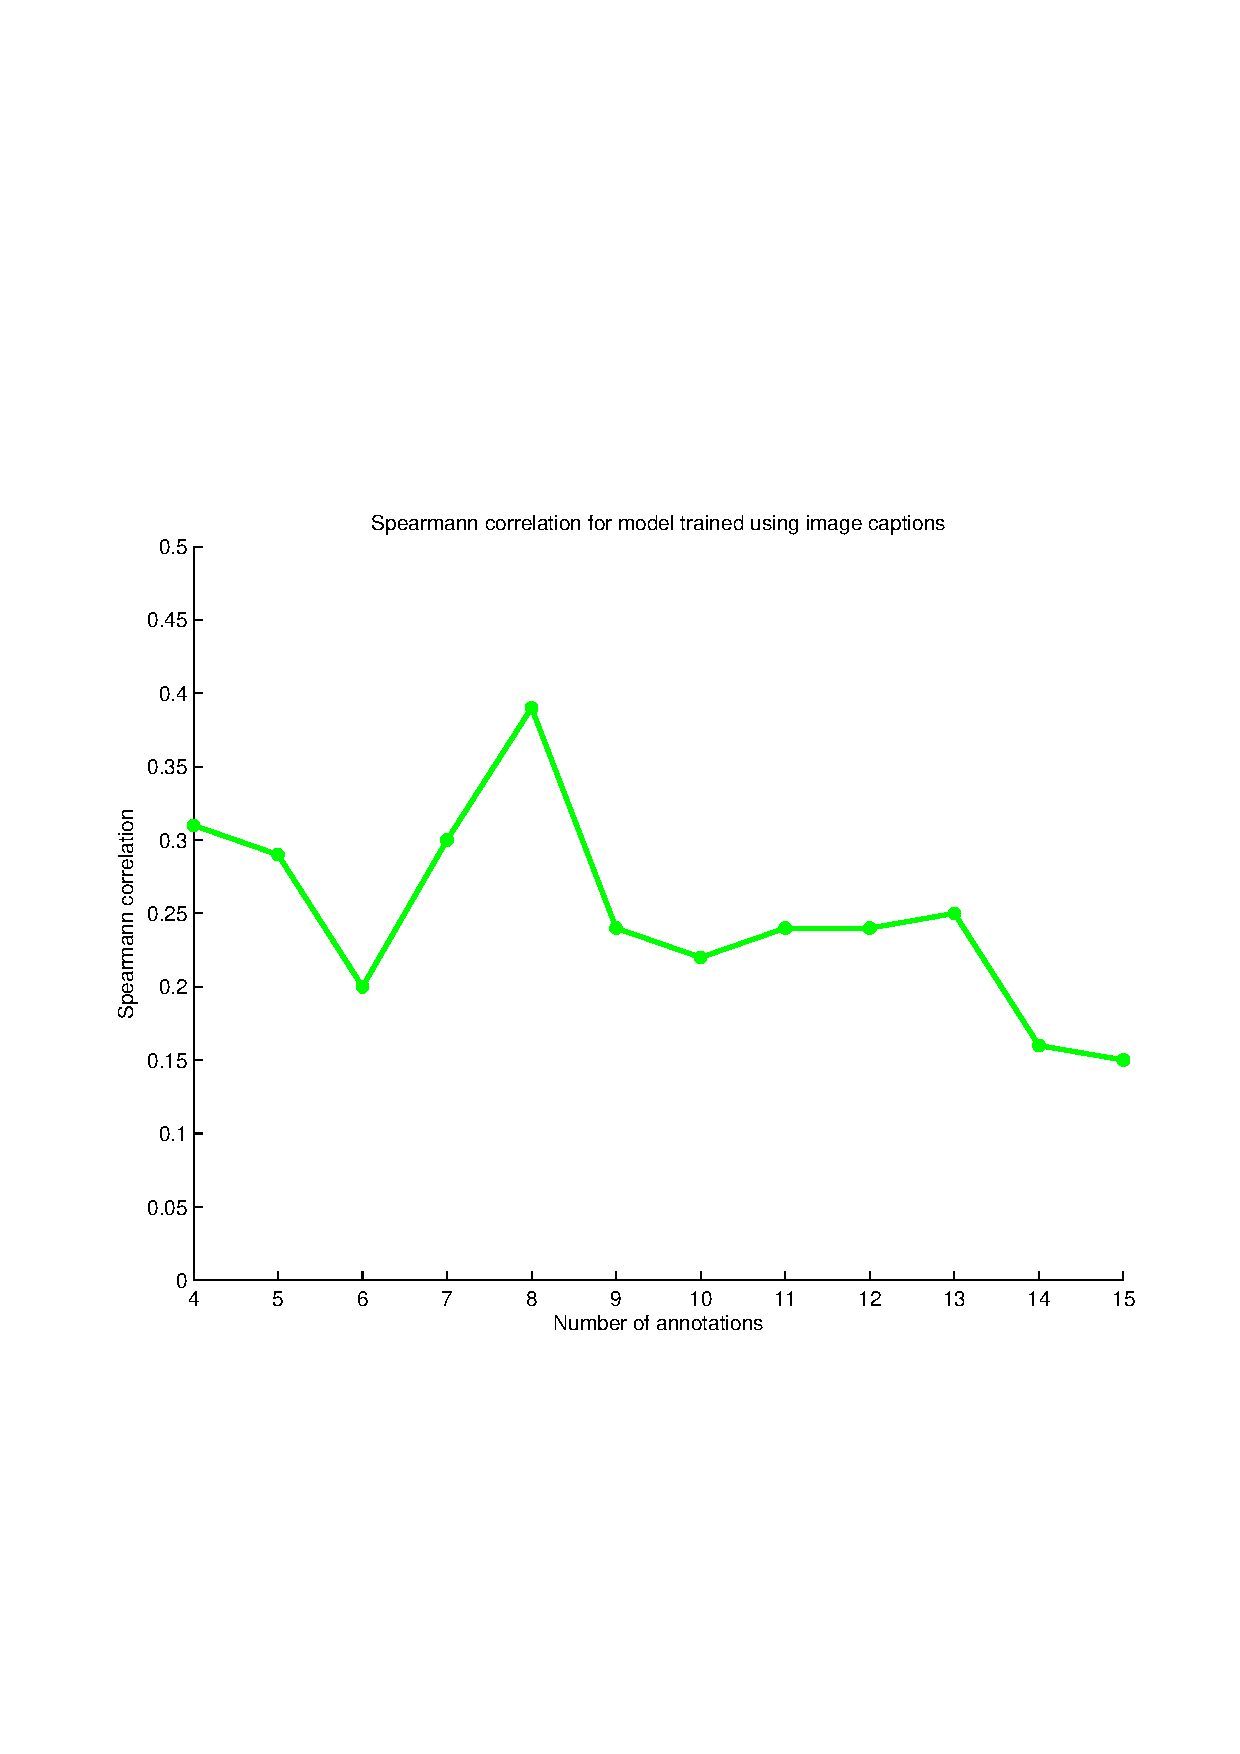
\includegraphics[width=0.7\columnwidth]{figures/annotations.pdf}
		\caption{Spearmann correlation on the validation set with models trained using image captioning features for varying number of annotations.}
    \label{num-ann}
\end{figure}

\begin{table*}
  \centering
  \renewcommand{\arraystretch}{1.2}
  \begin{tabular}{|c|c|c|c|c|c|c|}
    \hline
    \textbf{Feature} & \textbf{Feature type}& \textbf{Dimension}& \multicolumn{2}{c|}{\textbf{$SpCorr$($geq$ 4 annotations)}} & \multicolumn{2}{c|}{\textbf{$SpCorr$ ($geq$ 8 annotations)}}\\
    % \hline
    % \textbf{Inactive Modes} & \textbf{Description}\\
    \cline{4-7}
    & & & \emph{validation set}& \emph{test set} & \emph{validation set}& \emph{test set}\\ \hline
    C3D& visual spatio-temporal& 4096& 0.20& 0.26& 0.31& 0.34\\ \hline
		C3D (PCA)& visual spatio-temporal (PCA)& 225& 0.24& 0.21& 0.18& 0.17\\ \hline
		AudioSet& audio related& 128& 0.23& 0.22& 0.21& 0.24\\ \hline
		Affect& affect related& 400& 0.19& 0.17& 0.26& 0.23\\ \hline
		SentiBank concepts& emotion related& 300& 0.16& 0.13& 0.15& 0.17\\ \hline
		SentiBank features& emotion related& 4096& 0.25& 0.21& 0.27& 0.26\\ \hline
		SentiBank features (PCA)& emotion related (PCA)& 225& 0.22& 0.21& 0.22& 0.23\\ \hline
		Captions& visual-semantics & 300& 0.29& 0.31& 0.39& 0.38 \\ \hline
		Combination& combine-all-features (PCA)& 1578& 0.24& 0.23& 0.29& 0.27\\ \hline		
    \hline
  \end{tabular}
  \caption{Prediction results (Spearmann correlation) on validation and test data for different features with models trained on videos that have at least 4 (columns 4-5) or 8 (columns 6-7) annotations.}
	\label{res-4-10-ann}	
\end{table*}

These results are reported in the second part of Table \ref{res-4-10-ann}: $SpCorr$ ( $\geq$ 8 annotations).
Comparing the two sets of results in Table \ref{res-4-10-ann}, we observe that the models trained on sequences with at least 8 annotations perform better than the models trained on sequences with at least 4 annotations.
The only exception being the C3D (PCA) feature, where the model trained on sequences with at least 4 annotations performs marginally better than the model trained on sequences with at least 8 annotations. 
Additionally, we also observe that the scores for validation set and test set are very similar across the two sets of results.

%%%%%%%%%%%%%%%%%%%%%%%%%%%%%%%%%%%%%%%%%%%%%%%%%%%%%%%%%%%%%%%%%%%%%%%%%%%%%%%%%%%%%%%%%%%%%%%%%%%%%%%%%%%%%%%%%%%%%%%%%%%%%%%%%%%%%%%%%%%%%%%%%%%%%%%%%
\section{Conclusions}
%%%%%%%%%%%%%%%%%%%%%%%%%%%%%%%%%%%%%%%%%%%%%%%%%%%%%%%%%%%%%%%%%%%%%%%%%%%%%%%%%%%%%%%%%%%%%%%%%%%%%%%%%%%%%%%%%%%%%%%%%%%%%%%%%%%%%%%%%%%%%%%%%%%%%%%%%
%protocol
We proposed a new protocol to collect long-term memorability annotations for videos.
It enabled us to measure memory performance after weeks to years.
It appears from the analysis of the data that memory of videos continue to decrease for years, which justify a measurement of memory performance after a significant retention duration, longer than proposed in previous work.
The principal weakness of our protocol is the part of subjectivity susceptible to enter in our measure of memorability, that one should counteract by appropriate controls.
Our current work focus on collecting VM annotations at a large scale using crowdsourcing, measuring VM in a more objective manner.
The implemented protocol measure memory performance after two different retention durations, which will enable us to understand what makes a video lastingly memorable.

%modelling Karthik
After exploring a variety of generic (C3D, AudioSet), perceptual (SentiBank, Affect), and semantic (Image captions) features, we can say that a model trained with  semantic features provides predictions that are most correlated with ground-truth memorability scores.
It might be very interesting to investigate if these findings hold for generic video types other than movies.
Future research could involve investigating the memorability prediction performance on other generic videos using the existing set of features as well as other important features.
We also found that emotion features are not that well correlated with ground-truth memorability scores, as indicated in psychology literature.
An immediate direction for future research would be to explore other approaches to encode emotion in videos and investigate whether we can improve the prediction performance using these approaches.
We also investigated the number of annotations required to train a model and found a sweet spot where the performance is optimal.

%%%%%%%%%%%%%%%%%%%%%%%%%%%%%%%%%%%%%%%%%%%%%%%%%%%%%%%%%%%%%%%%%%%%%%%%%%%%%%%%%%%%%%%%%%%%%%%%%%%%%%%%%%%%%%%%%%%%%%%%%%%%%%%%%%%%%%%%%%%%%%%%%%%%%%%%%
\addtolength{\textheight}{-12cm}   % This command serves to balance the column lengths
                                  % on the last page of the document manually. It shortens
                                  % the textheight of the last page by a suitable amount.
                                  % This command does not take effect until the next page
                                  % so it should come on the page before the last. Make
                                  % sure that you do not shorten the textheight too much.
%%%%%%%%%%%%%%%%%%%%%%%%%%%%%%%%%%%%%%%%%%%%%%%%%%%%%%%%%%%%%%%%%%%%%%%%%%%%%%%%%%%%%%%%%%%%%%%%%%%%%%%%%%%%%%%%%%%%%%%%%%%%%%%%%%%%%%%%%%%%%%%%%%%%%%%%%

%%%%%%%%%%%%%%%%%%%%%%%%%%%%%%%%%%%%%%%%%%%%%%%%%%%%%%%%%%%%%%%%%%%%%%%%%%%%%%%%%%%%%%%%%%%%%%%%%%%%%%%%%%%%%%%%%%%%%%%%%%%%%%%%%%%%%%%%%%%%%%%%%%%%%%%%%
%\section*{Appendix}
%%%%%%%%%%%%%%%%%%%%%%%%%%%%%%%%%%%%%%%%%%%%%%%%%%%%%%%%%%%%%%%%%%%%%%%%%%%%%%%%%%%%%%%%%%%%%%%%%%%%%%%%%%%%%%%%%%%%%%%%%%%%%%%%%%%%%%%%%%%%%%%%%%%%%%%%%
 %Liste des features (comme/ceux de MediaEval 2015 à donner au téléchargement avec le début en sec de nos sequences)
 %Release text file for movie title, start/end time + features


%%%%%%%%%%%%%%%%%%%%%%%%%%%%%%%%%%%%%%%%%%%%%%%%%%%%%%%%%%%%%%%%%%%%%%%%%%%%%%%%%%%%%%%%%%%%%%%%%%%%%%%%%%%%%%%%%%%%%%%%%%%%%%%%%%%%%%%%%%%%%%%%%%%%%%%%%
%\section*{Acknowledgment}
%%%%%%%%%%%%%%%%%%%%%%%%%%%%%%%%%%%%%%%%%%%%%%%%%%%%%%%%%%%%%%%%%%%%%%%%%%%%%%%%%%%%%%%%%%%%%%%%%%%%%%%%%%%%%%%%%%%%%%%%%%%%%%%%%%%%%%%%%%%%%%%%%%%%%%%%%
%optional (%to acknowledge grants, funding, editing assistance and what have you.)

%%%%%%%%%%%%%%%%%%%%%%%%%%%%%%%%%%%%%%%%%%%%%%%%%%%%%%%%%%%%%%%%%%%%%%%%%%%%%%%%%%%%%%%%%%%%%%%%%%%%%%%%%%%%%%%%%%%%%%%%%%%%%%%%%%%%%%%%%%%%%%%%%%%%%%%%%
%% BIBLIOGRAPHY
%%%%%%%%%%%%%%%%%%%%%%%%%%%%%%%%%%%%%%%%%%%%%%%%%%%%%%%%%%%%%%%%%%%%%%%%%%%%%%%%%%%%%%%%%%%%%%%%%%%%%%%%%%%%%%%%%%%%%%%%%%%%%%%%%%%%%%%%%%%%%%%%%%%%%%%%%
\bibliographystyle{ACM-Reference-Format}
\bibliography{references} 

%%%%%%%%%%%%%%%%%%%%%%%%%%%%%%%%%%%%%%%%%%%%%%%%%%%%%%%%%%%%%%%%%%%%%%%%%%%%%%%%%%%%%%%%%%%%%%%%%%%%%%%%%%%%%%%%%%%%%%%%%%%%%%%%%%%%%%%%%%%%%%%%%%%%%%%%%
\end{document}